%! Author = WelJo
%! Date = 8/18/2026

\newpage


\section{Results and Evaluation}
\label{sec:results-and-evaluation}


The following section presents the empirical findings of the multi-tier simulation across the 336-hour flood horizon.
We evaluate how infrastructure coupling impacts integrated accessibility robustness ($RoA_{\text{Int}}$) and test hypotheses on resilience overestimation, buffer dynamics, and recovery lag.

\subsection{Scope and Methodological Baseline}
\label{subsec:scope-and-baseline}

Our Level~A (Road-Only) baseline yields $RoA_{\text{Int}} = 84.58\,\%$ and a systemic nadir of $RoA_{\text{Sys,min}} = 38.41\,\%$ during peak HQ100 inundation, diverging from the $70.1\,\%$ regional benchmark by Kaub et al.~\cite{kaub2024}.
While their study spans $26{,}853$ nodes and $44$ fire stations across surrounding rural counties, our model focuses on municipal Trier ($117\,\text{km}^2$, $5{,}817$ nodes, $12$ fire stations).
This focused scope eliminates peripheral highway bypasses and suburban redundancy, exposing core urban vulnerabilities.
Combined with localized hydrodynamics, Level~A establishes a realistic transport baseline to isolate compound utility coupling (Level~C).

\subsection{Multi-Tier Quantitative Results and Simulation Timeline}
\label{subsec:quantitative-results}


Table~\ref{tab:multi-tier-summary} summarizes aggregate metrics across all four complexity tiers, and Figure~\ref{fig:multi-tier-ts} illustrates the systemic accessibility timeline across five disaster phases:


\begin{enumerate}
    \item \textbf{Pre-Event ($0 \le t < 48\,\text{h}$)}: Undisrupted baseline conditions.
    \item \textbf{Rising Limb ($48 \le t < 144\,\text{h}$)}: Floodwaters rise ($9.00\,\text{m} \to 11.80\,\text{m}$), closing roads and submerging substations while buffers sustain operations.
    \item \textbf{HQ100 Peak Plateau ($144 \le t < 192\,\text{h}$)}: Buffer exhaustion forces facilities offline, reaching nadir ($38.41\,\%$ Level A vs.\ $37.29\,\%$ Level~C).
    \item \textbf{Recession Limb} ($192 \le t < 288\,\text{h}$): Floodwaters recede; Level A recovers synchronously with road clearance, while Level C remains incapacitated.
    \item \textbf{Post-Event Recovery} ($288 \le t \le 336\,\text{h}$): Level A fully restores at hour 288, while Level C displays a 48-h recovery lag from reboot delays.
\end{enumerate}

\vspace{-\topsep}

\begin{figure}
    \centering
    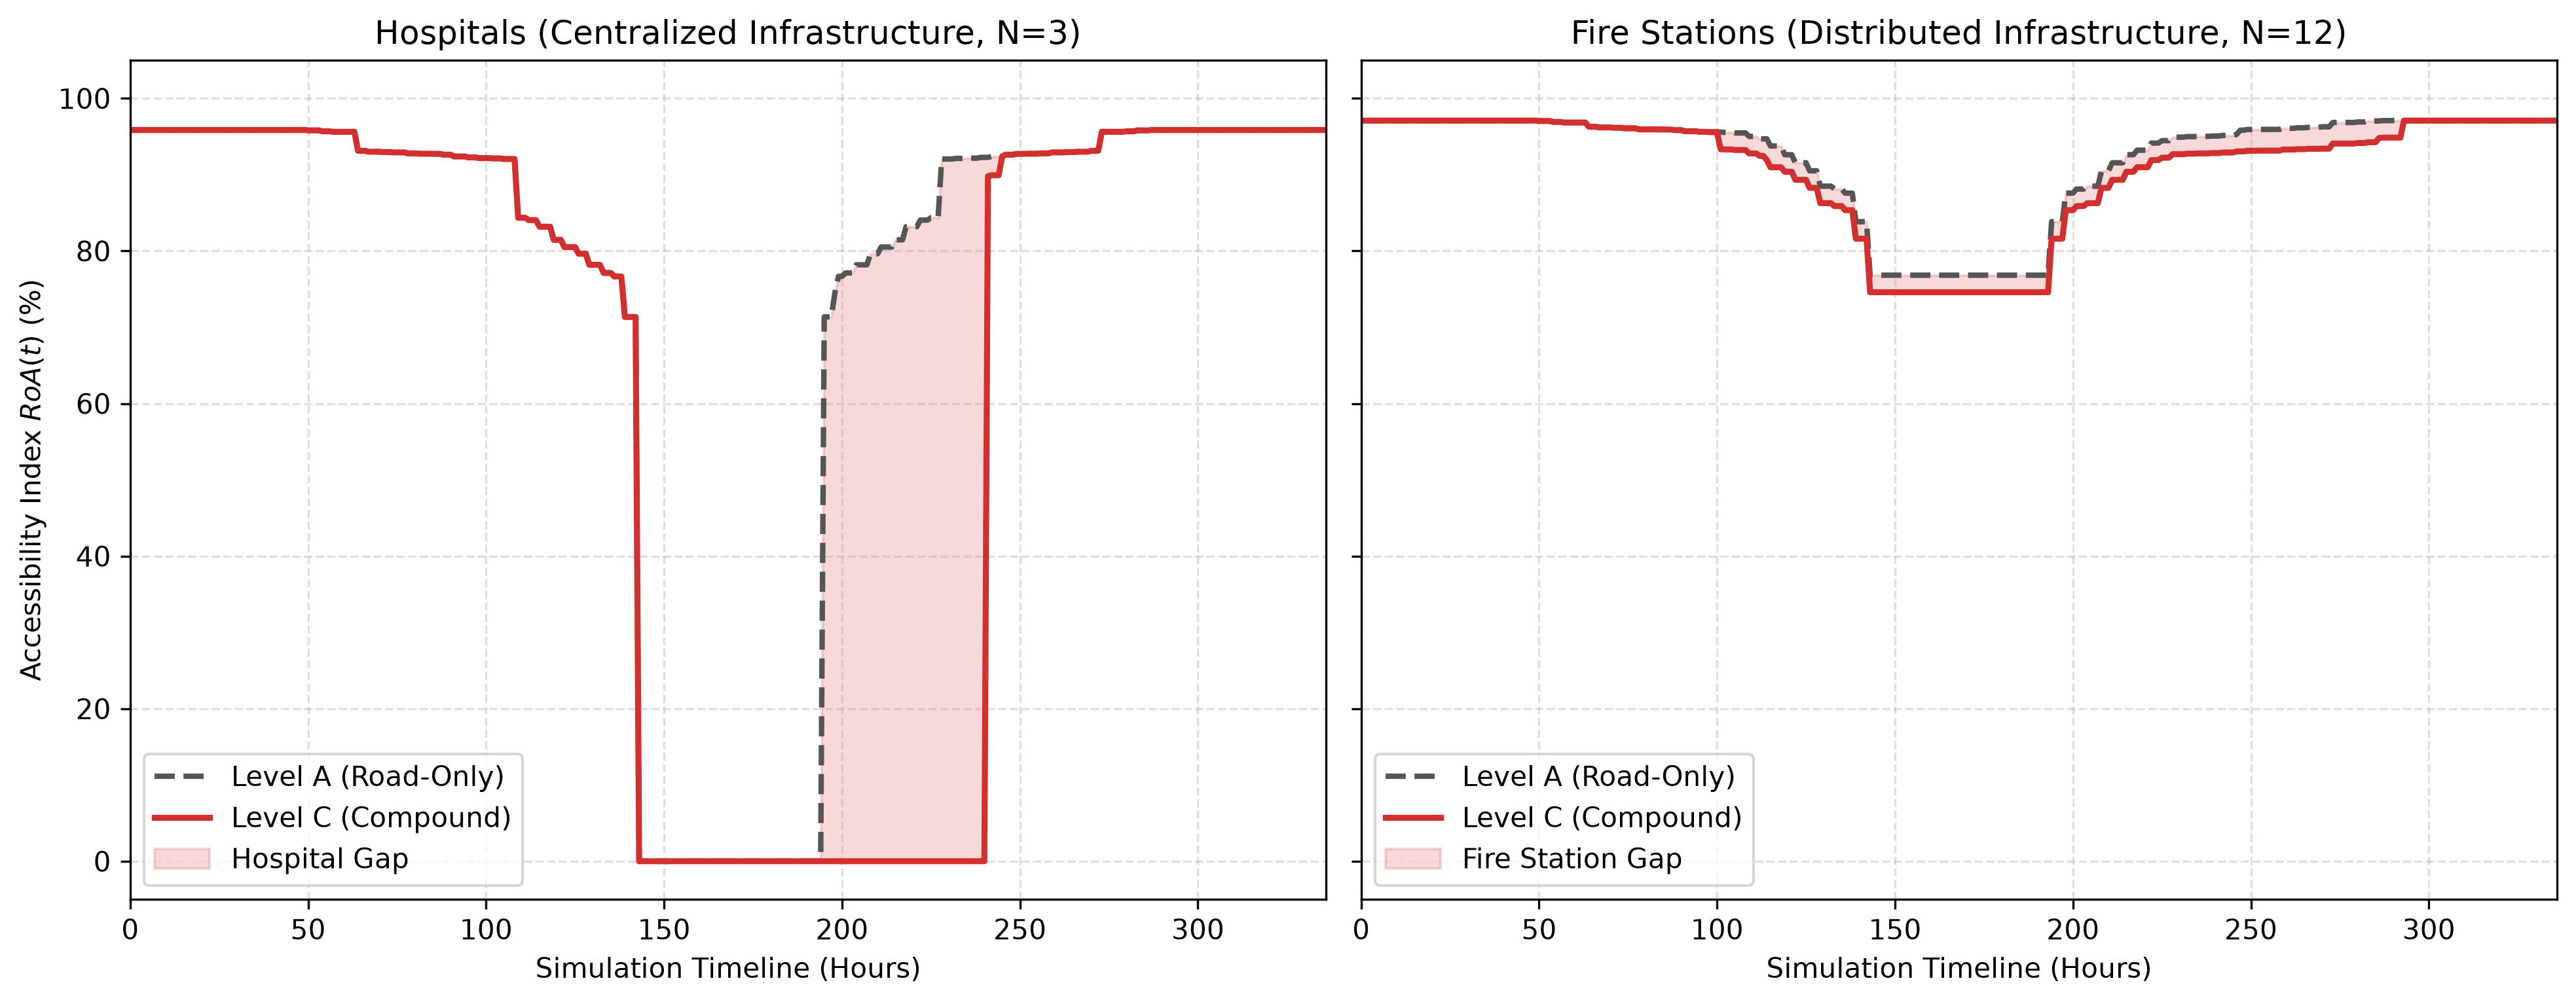
\includegraphics[width=0.76\linewidth]{resources/accessibility_comparison}
    \caption{Temporal evolution of $RoA$ for Level~A and Level~C over the 336-h horizon. Shading indicates the cumulative functional overestimation gap.}
    \label{fig:multi-tier-ts}
\end{figure}

\begin{table}[htbp]
    \centering
    \small
    \caption{Quantitative summary of multi-tier simulation results for Trier.}
    \label{tab:multi-tier-summary}
    \begin{tabularx}{\textwidth}{ >{\centering\arraybackslash}X >{\centering\arraybackslash}X >{\centering\arraybackslash}X >{\centering\arraybackslash}X >{\centering\arraybackslash}X }
        \hline
        \textbf{Level} & \textbf{$RoA_{\text{Int}}$} & \textbf{$RoA_{\text{Sys,min}}$} & \textbf{Hosp. Nadir} & \textbf{Fire Nadir} \\
        \hline
        Level A & $84.58\%$ & $38.41\%$ & $0.00\%$ & $76.82\%$ \\
        Level B1 & $78.20\%$ & $37.29\%$ & $0.00\%$ & $74.59\%$ \\
        Level B2 & $78.84\%$ & $38.41\%$ & $0.00\%$ & $76.82\%$ \\
        Level C & $78.20\%$ & $37.29\%$ & $0.00\%$ & $74.59\%$ \\
        \hline
    \end{tabularx}
\end{table}

\noindent
Intermediate tiers reveal power grid failure (Level~B1) as Trier's primary cascading bottleneck: Level~B1 matches Level~C identically ($RoA_{\text{Int}} = 78.20\,\%$, nadir $37.29\,\%$), whereas Level~B2 maintains higher resilience ($RoA_{\text{Int}} = 78.84\,\%$, nadir $38.41\,\%$). This indicates water networks are less vulnerable to flooding than power infrastructure.


\subsection{Hypothesis Testing and Validation}
\label{subsec:hypothesis-testing}

\subsubsection{Functional Gap and Resilience Overestimation}
\label{subsubsec:h1-analysis}
Hypothesis~H1 posits that transport-only models overestimate disaster resilience by ignoring cascading infrastructure dependencies.
This is confirmed: Level~C reveals a $1.12\,\%$ drop in peak nadir ($37.29\,\%$ vs.\ $38.41\,\%$) and a $6.38\,\%$ reduction in cumulative resilience ($RoA_{\text{Int}} = 78.20\,\%$ vs.\ $84.58\,\%$), demonstrating significant resilience overestimation.
The main contributors to this difference are the fire stations, where additional facilities are lost due to power outages, whereas hospitals lose all functionality across all levels due to inundation, as shown in Figures~\ref{fig:multi-tier-ts} and~\ref{fig:spatial-gap}.

\subsubsection{Temporal Buffers and Post-Flood Recovery Hysteresis}
\label{subsubsec:h2-analysis}
Hypothesis~H2 posits that facility buffers grant operational delay during onset, while restart requirements produce recovery hysteresis.
This is confirmed: emergency power buffers delay facility collapse by up to $24\,\text{hours}$ during flood rise.
This 48-hour recovery lag validates the operational penalty of FSM reboot latencies ($T_{\text{repair}} \in \{24\,\text{h for fire.}, 48\,\text{h for hosp.}\}$) and the $\theta = 0.15$ recharge threshold.

\subsection{Spatial Vulnerability: Municipal Patterns and Service Disparity}
\label{subsec:spatial-vulnerability}

To evaluate spatial disruption patterns across Trier, Figure~\ref{fig:spatial_resilience_map} maps accessibility loss ($\Delta RoA_j$) at peak flood (HQ100), comparing transport baseline (Level~A) against compound failure (Level~C).
River inundation severs primary transit arteries.
Because acute healthcare facilities ($N=3$) are clustered near the river axis, road closures eliminate access entirely, dropping hospital accessibility to $0.00\,\%$ across all tiers; hospital access is thus strictly transport-dominated.
Conversely, fire stations ($N=12$) are distributed across municipal districts, providing structural redundancy that preserves a $76.82\,\%$ nadir in Level~A.
Under Level~C, utility cascades compromise this distributed resilience, reducing fire station nadir to $74.59\,\%$, as shown in Figure \ref{fig:multi-tier-ts}

\begin{figure}
    \centering
    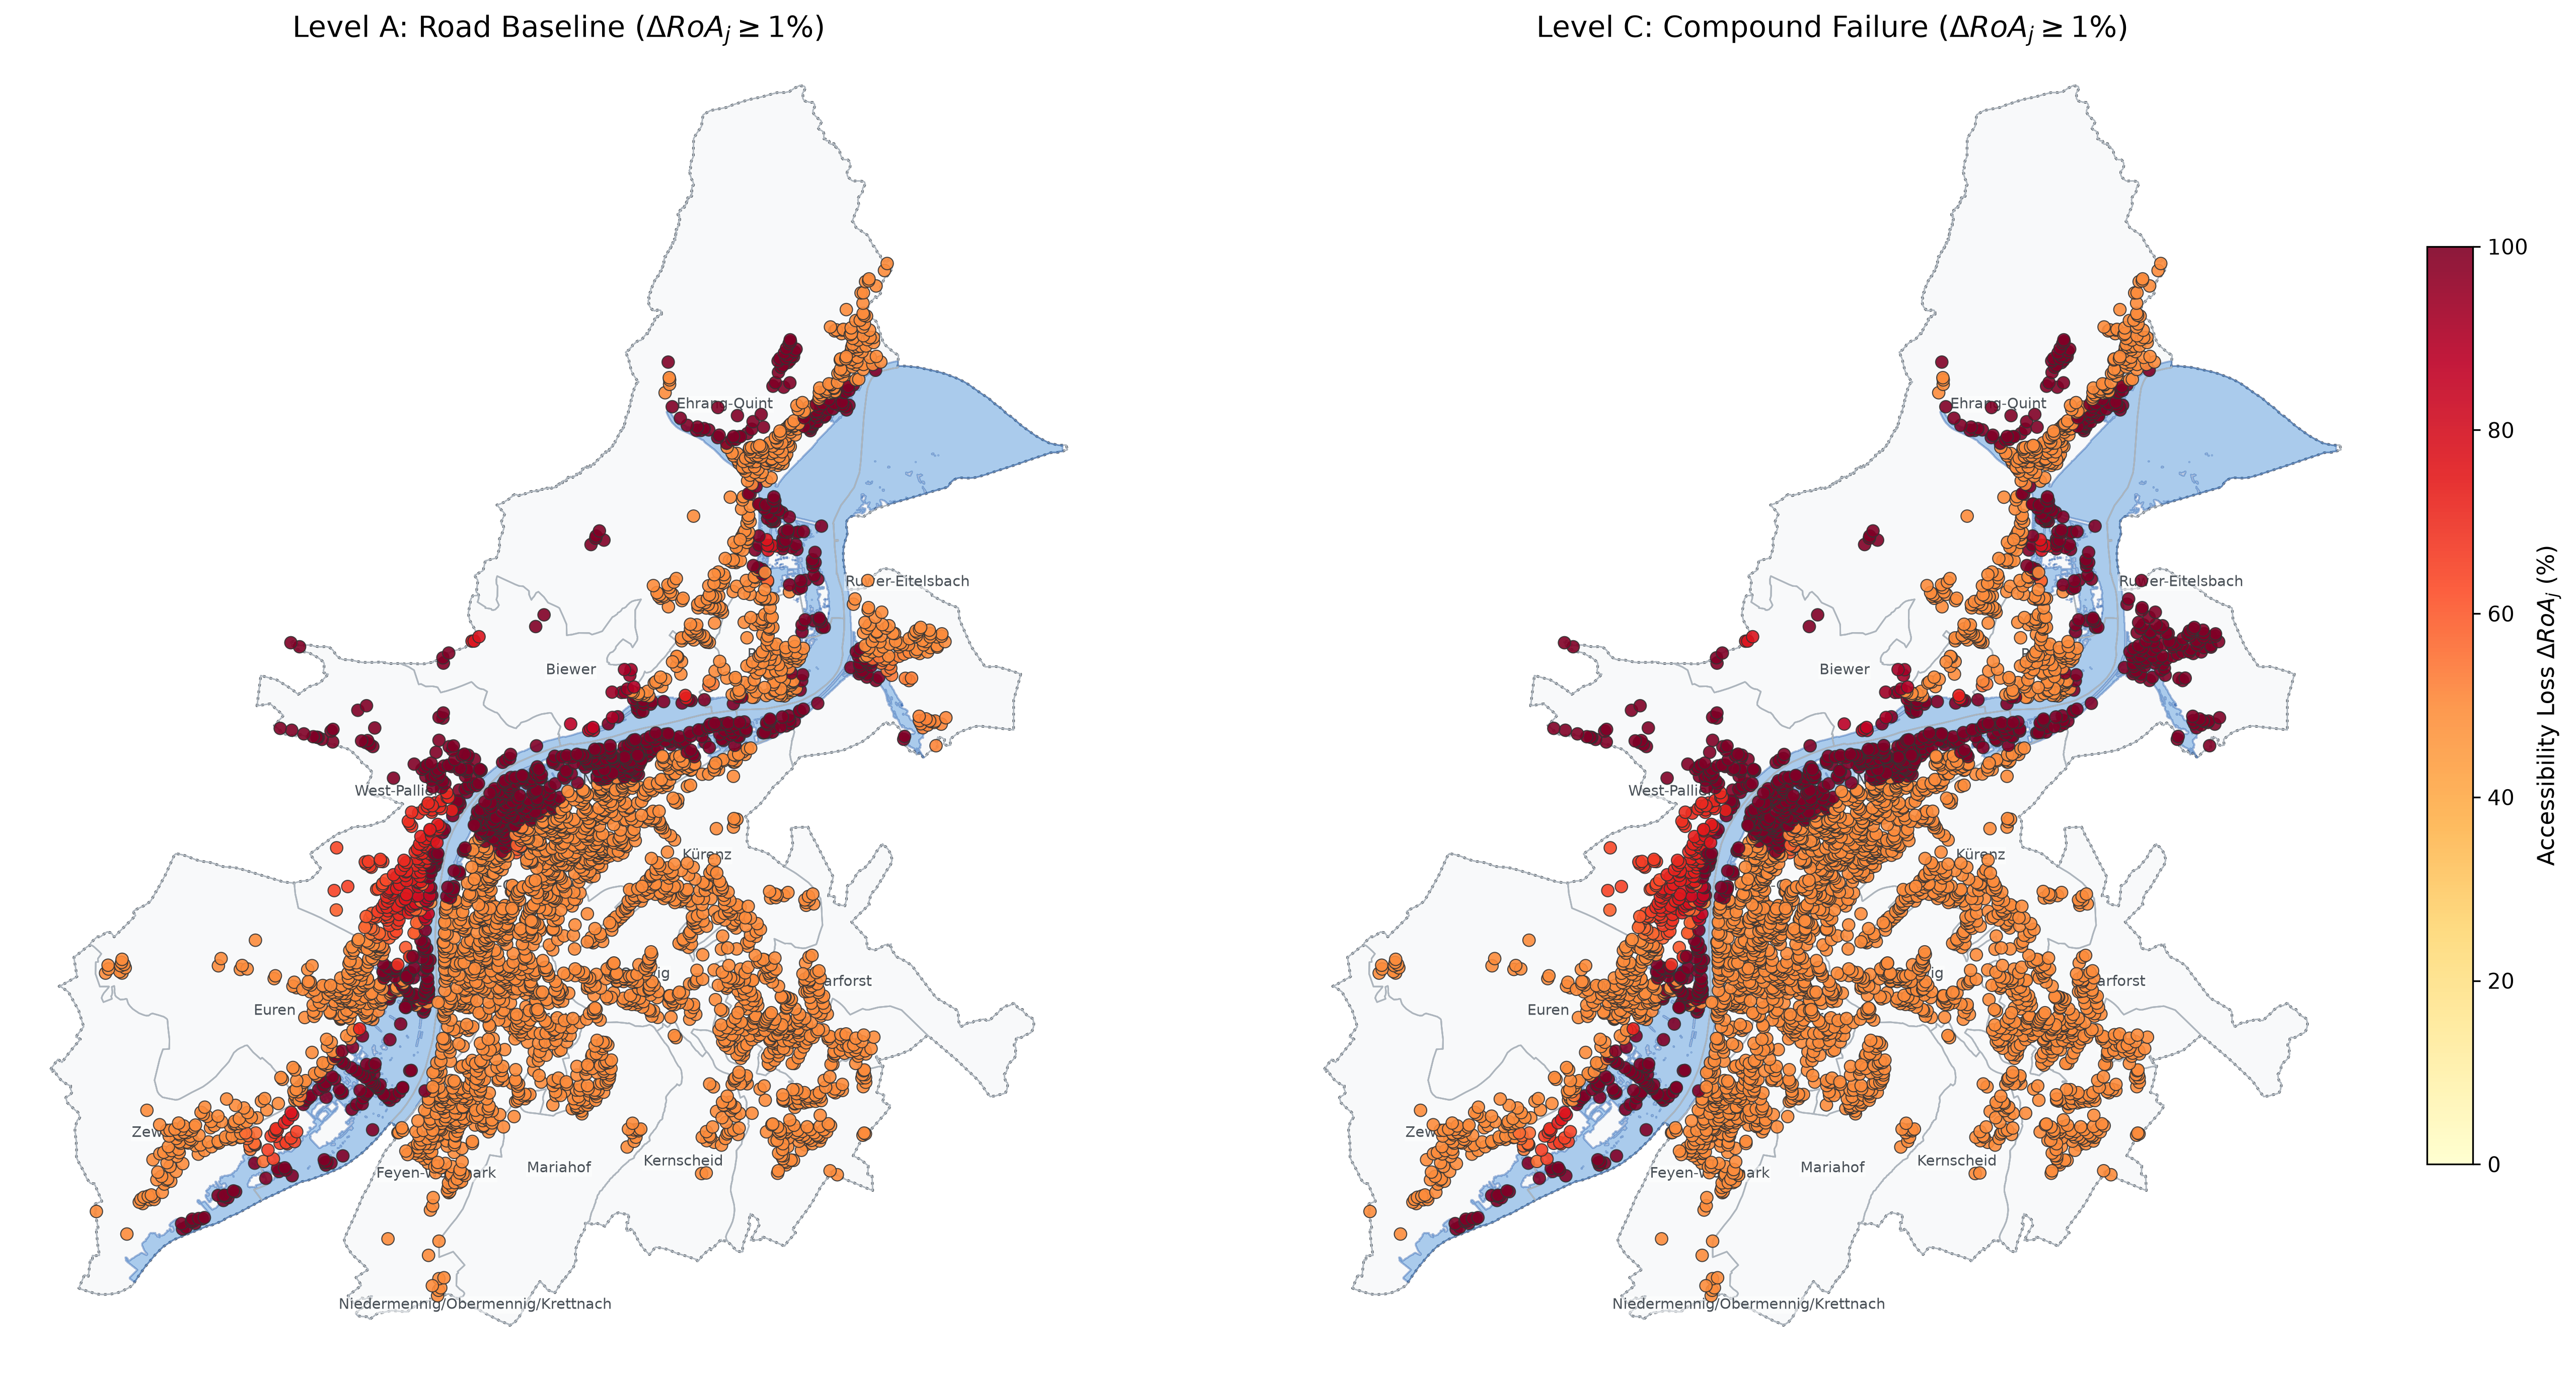
\includegraphics[width=0.63\linewidth]{resources/spatial_resilience_map}
    \caption{Spatial accessibility loss ($\Delta RoA_j$) across Trier at peak flood (HQ100): Level~A road baseline (left) vs.\ Level~C compound failure (right).}
    \label{fig:spatial_resilience_map}
\end{figure}

\vspace{-\topsep}

\subsection{District Vulnerability: The Ruwer-Eitelsbach Cascade}
\label{subsec:district-vulnerability}

District analysis reveals that divergence between Level~A and Level~C concentrates in Ruwer-Eitelsbach.
In all 18 other districts, the peak gap is negligible as facilities stay connected or are already road-isolated.
Ruwer-Eitelsbach exhibits a $31.99\,\%$ mean gap across 140 nodes (peaking at $50.00\,\%$, Figure~\ref{fig:spatial-gap}) via a four-step cascade:
(1)~\textbf{Topographical Immunity}: The local fire station stays dry above HQ100 (Level~A assumes $100\,\%$ operational).
(2)~\textbf{Off-Site Inundation}: In Level~C, its upstream valley substation submerges early during flood rise.
(3)~\textbf{Buffer Exhaustion}: After 24 hours, emergency generator fuel depletes, transitioning the station to \texttt{Dead}.
(4)~\textbf{Compound Cutoff}: Concurrently, arterial roads to central Trier submerge, leaving the district isolated.

\begin{figure}
    \centering
    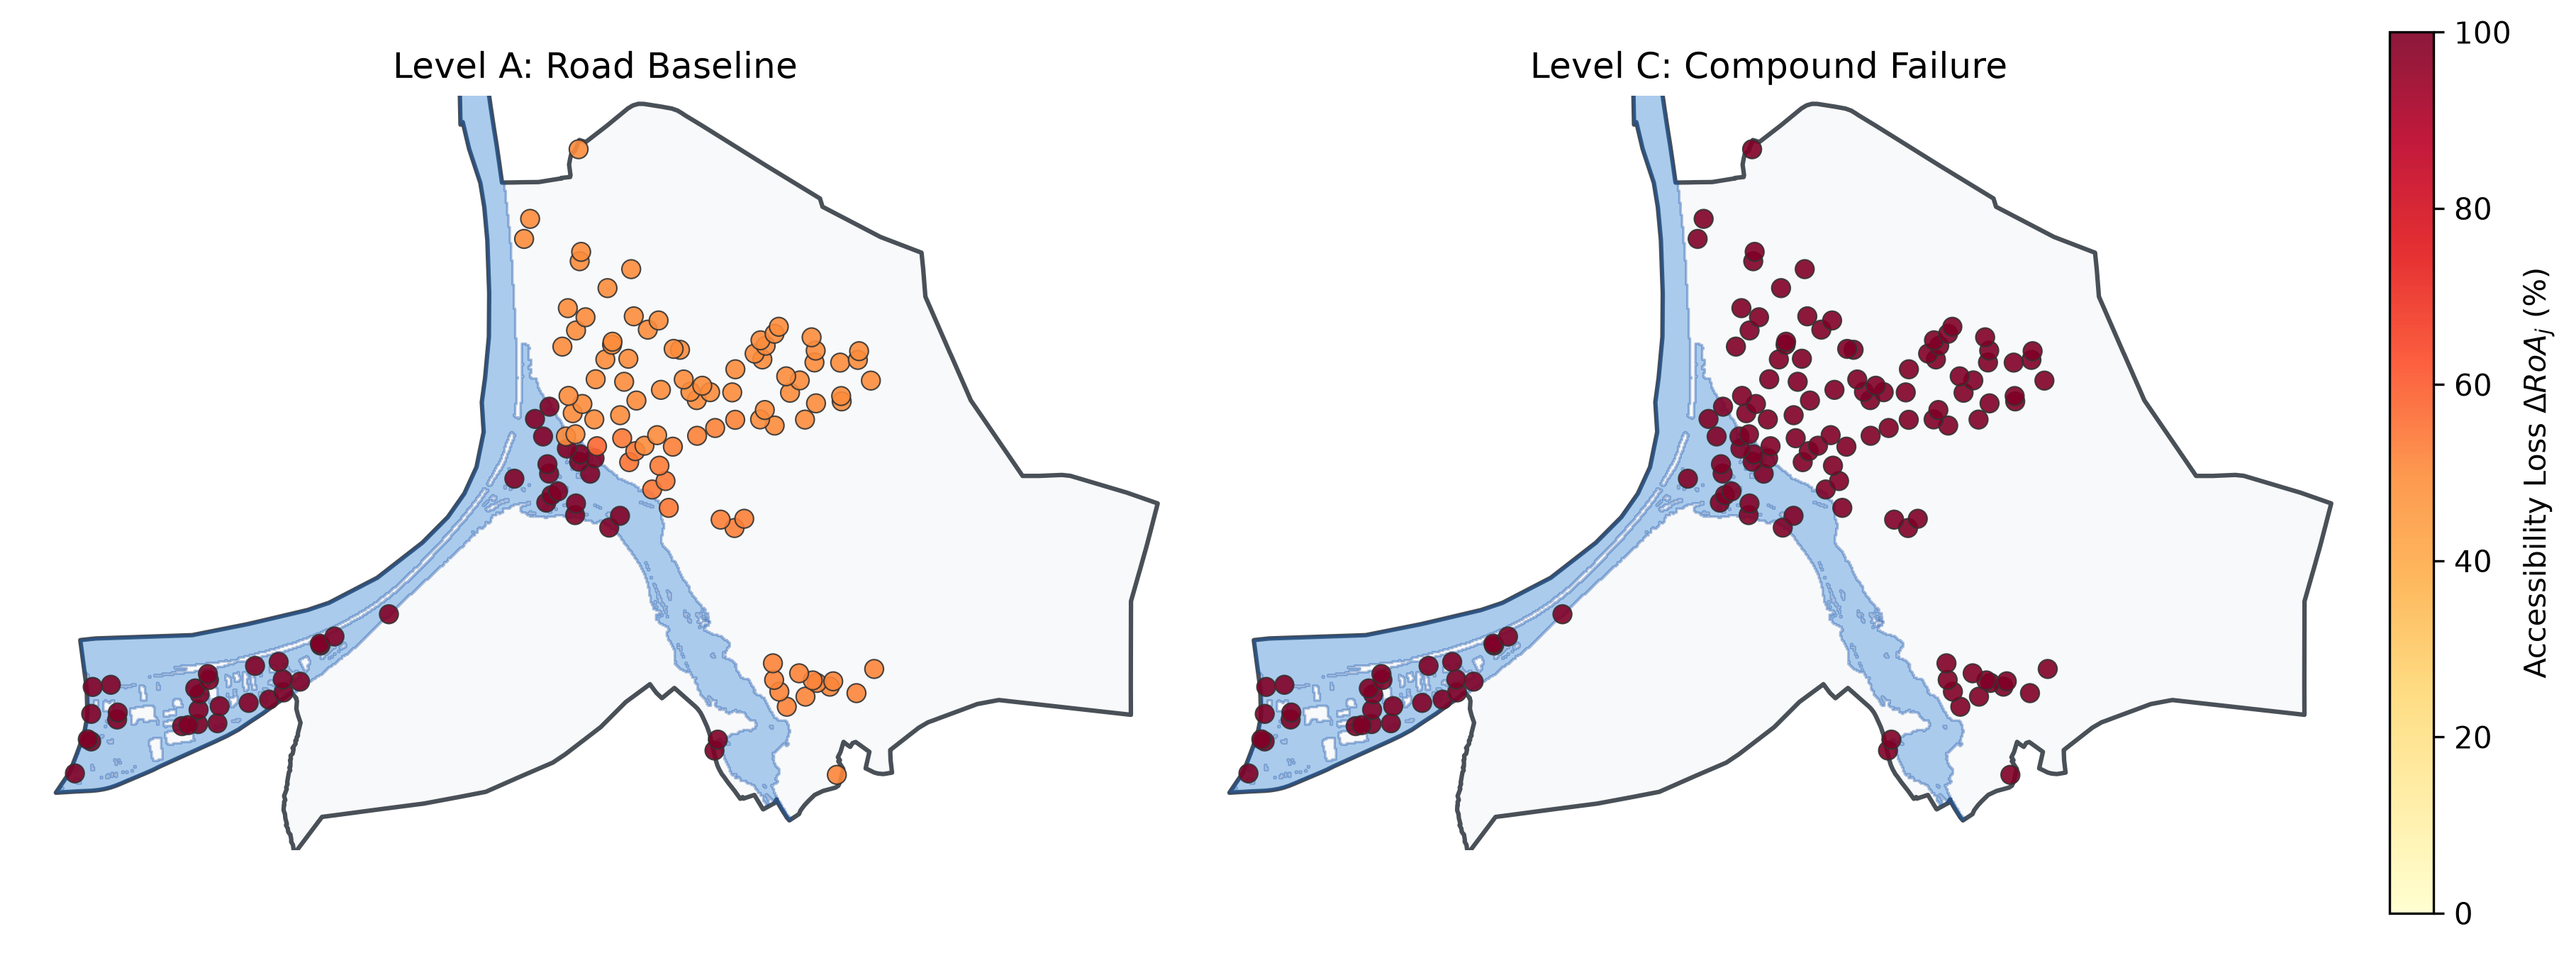
\includegraphics[width=0.62\linewidth]{resources/combined_resilience_map_ruwer}
    \caption{Heatmap of accessibility loss in Ruwer-Eitelsbach at peak flood: Level~A baseline (left) vs.\ Level~C compound failure (right).}
    \label{fig:spatial-gap}
\end{figure}

\vspace{-\topsep}

\subsection{Synthesis and Operational Implications}
\label{subsec:synthesis}

These empirical findings demonstrate that single-sector resilience models severely underestimate disaster risk.
By capturing infrastructure coupling, our framework exposes two critical blind spots: localized utility cascades in physically dry districts and a 48-hour restoration lag.
Emergency planners must therefore prioritize flood-hardened power feeds and sustained recovery refueling logistics.
